% !Mode:: "TeX:UTF-8"
\documentclass[preprint,authoryear,PhD]{cumtthesis}
\usepackage{listings}
\usepackage{multirow}
%\usepackage[left=3.17cm,right=3.17cm,top=3.0cm,bottom=3.0cm]{geometry}

%=================================== 数学符号 =================================%
\newcommand{\rtn}{\mathrm{\mathbf{R}}}
\newcommand{\N}{\mathrm{\mathbf{N}}}
\newcommand{\AS}{~\mathrm{a.s.}}
\newcommand*{\PR}{\mathrm{\mathbf{P}}}
\newcommand*{\EX}{\mathrm{\mathbf{E}}}
\newcommand*{\dif}{\,\mathrm{d}}
\newcommand*{\F}{\mathcal{F}}
\newcommand*{\prs}{\dif\PR-\mathrm{a.s.}}
\newcommand*{\pts}{\dif\PR\times\dif t-\mathrm{a.e.}}
\newcommand{\Ito}{It\^{o}}
\newcommand{\tT}[1][0]{[#1,T]}
\newcommand{\intT}[2][T]{\int^{#1}_{#2}}
\newcommand{\s}{\mathcal{S}}
\newcommand{\me}{\mathrm{e}}
\newcommand{\one}[1]{{\bf 1}_{#1}}
\newcommand{\Mm}{{\rm M}}
\DeclareMathOperator*{\sgn}{sgn}
%=================================== 数学符号 =================================%

\makeindex

\begin{document}
\frontmatter

%--------输入中文论文题目
\CLunWenTiMu{中国矿业大学硕博毕业论文 \LaTeX{} 模板 V2.0 (2015/08/04)}

%--------输入英文论文题目
\ELunWenTiMu[0.95]{China University of Mining and Technology \LaTeX{} Thesis Template V2.0 (2015/08/04)}

%--------输入论文作者
\ZuoZhe{肖立顺}

%--------输入导师职称,导师姓名
\DaoShi[教授]{范胜君}
\DiErDaoShi[教授]{江龙}

%--------输入毕业时间
\BiYeShiJian{2013}{10}

%--------输入中图分类号
\ZhongTuFenLeiHao{O211.5}

%--------输入UDC
\UDC{519.2}

%--------输入密级
\MiJi{公开}

%--------输入毕业学校, 默认是中国矿业大学
%\BiYeXueXiao{}

%--------输入学校代码, 默认是10290
%\XueXiaoDaiMa{}

%--------输入学位类别
\XueWeiLeiBie{理学}

%--------输入培养单位
\PeiYangDanWei{理学院}

%--------输入学科专业
\XueKeZhuanYe{概率论与数理统计}

%--------输入研究方向
\YanJiuFangXiang{随机分析}

%--------输入答辩委员会主席
\DaBianWeiYuanHuiZhuXi{江龙}

%--------输入评阅人
\PingYueRen{江龙, 周圣武}

%--------制作封面命令
\makecover

%--------致谢
\begin{acknowledgements}
  从 2011 年开始制作 cumtthesis.cls 的第一个版本, 到 2015 年的 V2.0 版本, 花费了大量的时间和精力, 期间得到了很多好心人的帮助.

  编写 cumtthesis.cls 中图表清单的代码时, \href{http://tex.stackexchange.com/}{酷 \LaTeX{} 问答站} 的 egreg
  帮我解决了关键性的技术问题, 并且很耐心很及时地解答我的疑问.

  我是看了薛瑞尼制作的 thuthesis.dtx 源代码才开始琢磨如何``文学式"编程. 从薛瑞尼的代码和
  文档中, 我得到了很多启发. 比如图表标题的制作, 比如变量注释表的代码编写, 还比如
  \verb|*.dtx| 文档的制作等.

  cumtthesis.cls 中双语目录的编写受哈尔滨工业大学硕博士学位论文 \LaTeX{} 模板 (1.9.2.20090324 版) 的启发,
  通过 \verb|*.toe| 文件来生成英语目录.

  第 \ref{cha:IntroductionOfTeX} --  \ref{cha:ResumesOfSupermans} 章的演示内容复制于
  \href{http://zzg34b.w3.c361.com/}{\LaTeX{} 编辑部}.
\end{acknowledgements}

%--------中文摘要
\begin{cabstract}
本文是对 cumtthesis.cls 模板的演示, 体现模板的各种功能. 制作 cumtthesis.cls
的目的是给矿大学子提供一个简洁易用的毕业论文模板, 宗旨是让使用者只关心论文的内容
而不用关心论文的格式.

本文总共有图 \ref{totalfigure} 幅, 表 \ref{totaltable} 张, 参考文献 \ref{totalbib} 篇.

%--------中文关键词
\CKeyWords{
\LaTeX; 模板; 中国矿业大学; 硕博论文; Word; 宏包;
cls 文档; 代码; 默认格式; 参考文献; 双语标题; 双语目录; 页面边距; 定理;
定义; 交叉引用.}
\end{cabstract}

%--------英文摘要
\begin{eabstract}
This paper is an illustration of cumtthesis.cls, which can reflect the various
functions of the template. The purpose of cumtthesis.cls is to provide a
simple and easy-to-use thesis template for cumters. It allows users to only
care about the content of the papers rather than the format.

There are totaly \ref{totalfigure} figures, \ref{totaltable} tables and \ref{totalbib} references
in this paper.

%--------英文关键词
\EKeyWords{\LaTeX; CUMT; Thesis of MD and PhD; Word; Package; cls document;
Codes; Default format; References; Bilingual titles; Bilingual contents;
Page margins; Theorem; Definition; Cross reference.}
\end{eabstract}

%-------英文拓展摘要
\begin{exabstract}
This paper is an illustration of cumtthesis.cls, which can reflect the various
functions of the template. The purpose of cumtthesis.cls is to provide a
simple and easy-to-use thesis template for cumters. It allows users to only
care about the content of the papers rather than the format.

There are totaly \ref{totalfigure} figures, \ref{totaltable} tables and \ref{totalbib} references
in this paper.

%--------英文拓展关键词
\ExKeyWords{\LaTeX; CUMT; Thesis of MD and PhD; Word; Package; cls document;
Codes; Default format; References; Bilingual titles; Bilingual contents;
Page margins; Theorem; Definition; Cross reference.
}
\end{exabstract}




%--------插入中文目录
\tableofcontents
%--------插入英文目录
\tableofecontents

%--------插入图清单
\listoffigures
%--------插入表清单
\listoftables
%--------变量注释表

\begin{notation}[2.5cm]
\item[$P$] 概率
\item[$\mathcal{F}$] 域流
\item[cumtthesis.ins] 模板的分解文件
\item[cumtthesis.dtx] 模板的说明文件
\item[cumtthesis.pdf] 模板的使用说明
\item[cumtthesis.cls] 模板的文档类
\item[cumtthesis.cfg] 文档类的配置文件
\item[cumt.bst] 矿大参考文献样式
\item[.tex] 示例文档代码
\item[.pdf] 示例文档
\item[.aux] 引用标记记录文件, 用于再次编译时生成参考文献和超链接等
\item[.bbl] 由 BibTeX 编辑 .bib 后创建的文献文件, 再次编译时带入源文件生成文献列表
\item[.blg] BibTeX 处理过程记录文件
\item[.dvi] 由 \LaTeX{} 对 .tex 源文件编译后创建的输出文件, 含有字库信息
\item[.glo] 术语标记记录文件, 用于再次编译时生成术语表
\item[.idx] 索引资料记录文件, 可用 makeindex 排序后创建索引文件 .ind
\item[.ilg] makeindex 处理过程记录文件
\item[.ind] makeindex 对 .idx 排序后创建的索引文件, 再次编译时带入源文件生成索引
\item[.lof] 图形标题记录文件, 用于再次编译时生成图形目录
\item[.log] 编译过程记录文件, 记录编译时出现的提示, 警告和错误信息
\item[.lot] 表格标题记录文件, 用于再次编译时生成表格目录
\item[.toc] 中文章节标题记录文件, 用于再次编译时生成中文章节目录
\item[.toe] 英文章节标题记录文件, 用于再次编译时生成英文章节目录
\item[\bf 英雄本色] 我等这个机会等了三年, 不是为了证明我比别人强, 只是要证明我失去的
    东西, 我一定要夺回来.
\item[\bf 临江仙 (杨慎)]滚滚长江东逝水, 浪花淘尽英雄, 是非成败转头空, 青山依旧在, 几度
    夕阳红. 白发渔樵江渚上, 惯看秋月春风. 一壶浊酒喜相逢, 古今多少事, 都付笑谈中.
\item[\bf 大话西游] 曾经有一份真诚的爱情摆在我的面前, 我没有珍惜, 等到失去的时候才追悔
    莫及, 人世间最痛苦的事情莫过于此. 如果上天能够给我一个重新来过的机会, 我会对那
    个女孩子说三个字:``我爱你". 如果非要给这份爱加上一个期限, 我希望是, 一万年.
\item[\bf 喜剧之王] 你可以说我是跑龙套的, 但是你不可以说我是``臭跑龙套"的.
\item[\bf 东邪西毒] 当你不能够再拥有, 你唯一可以做的, 就是令自己不要忘记.
\item[\bf 纵横四海] 其实爱一个人并不是要跟她一辈子的. 我喜欢花, 难道你摘下来让我闻;
    我喜欢风, 难道你让风停下来; 我喜欢云, 难道你就让云罩着我; 我喜欢海, 难道我就去
    跳海?
\item[\bf 无间道] 往往都是事情改变人, 人却改变不了事情.
\item[\bf 笑傲江湖] 有人就有恩怨, 有恩怨就有江湖. 人就是江湖, 你怎么退出!
\item[\bf 泰坦尼克号] 我甚至连他的一张照片都没有, 他只活在我的记忆里.
\item[\bf 似水年华] 一个男人和一个女人, 他们在完全对对方没有任何了解和认识的情况下,
    竟然会在一个清晨, 拥抱在一起. 他们在渴求的是什么? 他们不是在要对方, 他们在要自
    己. 我们在所有经过的爱情当中, 都不是看到的对方, 只是看到了自己.
\end{notation}

%================================== 正文开始 ==================================%
\mainmatter

\chapter{\TeX{} 简介}{Introduction of \TeX}
\label{cha:IntroductionOfTeX}

\TeX{} \index{\TeX} 是一个格式化排版系统, 它一问世便以其排版效果的高质量震动整个
出版界. 尤其是在排版含有大量数学公式的科技文献方面更显示了它的优越性. \TeX{}
\index{\TeX} 还是一个程序源代码公开的免费排版系统, 因此吸引了许多计算机专家及
\TeX{} \index{\TeX} 爱好者为之添砖加瓦.

20 世纪 60 年代, 著名计算机专家和数学家, 斯坦福大学 Donald E. Knuth \index{Knuth}
(读音: ka-nooth) 教授准备出系列专著《The art of computer programming》, 前三卷已
经出版. 当他正在撰写第四卷时, 出版社拿来了第二卷的第二版书样给他过目, 结果令他大
失所望, 因为当时出版社的印刷技术没有使他的书稿更好看, 反而变糟了, 尤其是在数学公
式和字体上面的缺陷更令他无法接受. 于是他就打算自己写一个既能供科学家编排手稿又符
合出版社印刷要求的高质量的计算机排版系统 \index{计算机排版系统}.

\begin{figure}
  \centering
  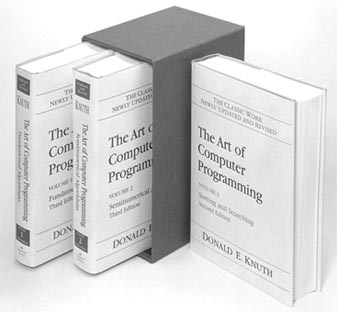
\includegraphics[width=6cm]{TheArtOfComputerProgramming.jpg}\\
  \caption{计算机编程的艺术}{The art of computer programming}
  \label{fig:TheArtOfComputerProgramming}
\end{figure}

Knuth \index{Knuth} 教授于 1977 年开始构造 \TeX{} \index{\TeX} 系统, 并为该系统
设计了一个字符字体生成软件: METAFONT\index{METAFONT}, 在标准的 \TeX{} \index{\TeX}
系统中包含有 75 种不同尺寸的字体, 且每种字体有 8 种不同的缩放比例.

1982 年 \TeX{} \index{\TeX} 系统成功开发出版, 之后又有几次升级. Knuth \index{Knuth}
教授用无理数 $\pi$ 的近似值作为 \TeX{} \index{\TeX} 系统的版本序号, $\mathrm{e}$
的近似值作为 METAFONT \index{METAFONT} 版本序号, 每升级一次其版号就增加一位数字,
不断地趋近于 $\pi$ 和 $\mathrm{e}$, 这也表达了 \TeX{} \index{\TeX} 不断追求完美
的愿望.

\TeX{} \index{\TeX} 的名称是由三个大写的希腊字母 $\tau\epsilon\chi$ 组成, 在希腊
语中这个词是``科学"和``艺术"的意思. 为了方便的缘故, 一般都写成 ``TeX", 念做
``teck". 更多关于 \TeX{} \index{\TeX} 的介绍可以参考 Knuth \index{Knuth} 教授编
写的《The TeXbook》(\cite{Knuth1984}).

\TeX{} \index{\TeX} 系统的内核相当稳定, 几乎没有 bug, 1995 年以后版本号一直停止
在 3.14159, 直到 2002 年 12 月才又进行了一次升级. 到目前为止, \TeX{} \index{\TeX}
系统的版本序号是 3.141592, METAFONT \index{METAFONT} 版本序号为 2.71828. 所以
Knuth \index{Knuth} 教授非常自信地说: ``I believe that the final bug in \TeX{}
\index{\TeX} was discovered and removed on November 27, 1985. But if,
somehow, an error still lurks in the code, I shall gladly pay a finder's fee of
\$20.48 to the first person who discovers it. (This is twice the previous amount,
and I plan to double it again in a year; you see, I really am confident!)"

\begin{figure}
  \centering
  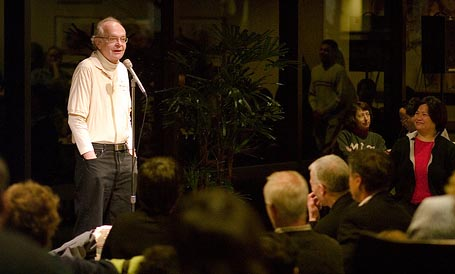
\includegraphics[width=8cm]{KnuthSpeech1990.jpg}\\
  \caption{Knuth \index{Knuth} 在 1990 年发出最终宣言}{Knuth gave the final declaration in 1990}
  \label{fig:KnuthSpeech1990}
\end{figure}


1990 年 \TeX{} \index{\TeX} 第 3.1 版发布时 (\cite{BaoTaiLei2008}), Knuth \index{Knuth} 教授发出最终宣言:
\begin{itemize}
  \item 不再对 \TeX{} \index{\TeX} 进行任何扩张;
  \item 如果出现明显问题, 修正的版本依次为 3.14 版, 3.141 版, 3.1415 版 \ldots,
        在自己离开这个世界的时候, 将最后的 \TeX{} \index{\TeX} 版本序号改为 $\pi$.
        此后, 即使再发现错误, 也都将成为 \TeX{} \index{\TeX} 的特征而保留. 如果
        有人非要修改的话, 就不要再叫 \TeX{} \index{\TeX} 了, 请另外起名.
  \item 关于 \TeX{} \index{\TeX} 的一切, 已经全部做了书面说明, 可以自由利用设计
        其他的软件.
\end{itemize}

\TeX{} \index{\TeX} 系统是由 Pascal \index{Pascal} 语言编写的, 程序的源代码也是
公开的. 它包含 300 条基本命令和 600 条扩展命令, 几乎可以排版任何形式的文献, 如一
般文章、报告、书刊和诗集等, 对数学公式的排版也被公认是最好的. \TeX{} \index{\TeX}
系统的优点之一就是它支持命令宏, 这使得使用 \TeX{} \index{\TeX} 成为一种乐趣, 用户
可以自己编写宏包来定义更多、更方便的新命令, 这也是 \TeX{} \index{\TeX} 能得以迅速
发展的原因. 而且, \TeX{} \index{\TeX} 是一个可移植的软件系统, 它可以运行于所有类
型的计算机 (如苹果机、IBM PC 机及大型工作站) 和各种操作系统 (如 DOS、Windows、
Unix 等).

\TeX{} \index{\TeX} 另一个重要特征就是它的输出是与设备无关. \TeX{} \index{\TeX}
的输出文件称为 DVI 文件, 即是``设备无关". 一旦 \TeX{} \index{\TeX} 处理了你的文
件, 所得到的 DVI 文件就可以被送到任何输出设备如打印机、屏幕等, 并且总会得到相同
的结果, 而这与这些输出设备的限制没有任何关系. 这说明 DVI 文件中所有的元素, 从页
面设置到文本中字符的位置都被固定, 不能更改.

最基本的 \TeX{} \index{\TeX} 程序只是由一些很原始的命令组成, 它们可以完成简单的
排版操作和程序设计功能. 然而, \TeX{} \index{\TeX} 也允许用这些原始命令定义一些更
复杂的高级命令. 这样就可以利用低级的块结构, 形成一个用户界面相当友好的环境.

虽然 \TeX{} \index{\TeX} 在过去的二十多年中没有大的变化, 但它开放的设计使得它能
够很容易适应新的要求.  例如, 在没有改动内核的情况下, \TeX{} \index{\TeX} 很容易
地实现了对 PostScript\index{PostScript} 字体和外部图形的支持; \TeX{} \index{\TeX}
是第一个能够自动生成 HTML 的字处理软件; 现在, \TeX{} \index{\TeX} 还可以在不
借助其它工具 (如 Adobe Distiller) 的条件下生成 PDF 格式文件.

\TeX{} \index{\TeX} 不仅是一个排版程序, 而且是一种程序语言. \LaTeX{} \index{\TeX}
就是使用这种语言写成的一个``\TeX{} \index{\TeX} 宏包", 它扩展了 \TeX{} \index{\TeX}
的功能, 使我们很方便地进行富于逻辑性的创作而不是专心于字体、缩进等这些烦人的东西.

\TeX{} \index{\TeX} 源文件是 ASCII 码文件, 可以方便地在网络上传播. 目前, 大多数
学术部分和校园网上都安装有 \TeX{} \index{\TeX} 系统. 国际上许多出版机构也采用
\TeX{} \index{\TeX} 系统来排版书刊, 不少出版社还要求作者提供稿件的 \TeX{} \index{\TeX}
源文件.

\chapter{\TeX{} 的优缺点}{The Advantages and Disadvantages of \TeX}

在一个充斥着``所见即所得"桌面出版软件的情况下来使用 \TeX{} \index{\TeX} 确是有点
令人奇怪. 但是, 在某些情形下, 你会感到 \TeX{} \index{\TeX} 是最好的, 甚至是唯一
适合的系统.

首先我们来看一下 \TeX{} \index{\TeX} 的优势所在:

\begin{description}
  \item[高质量的输出] \TeX{} \index{\TeX} 遵循传统的排版规则, 以排版质量为最重
       要的目标. 如果把 \TeX{} \index{\TeX} 的输出结果和用其它的排版软件排版相同
       的文本所得到的结果加以比较, 就会发现其中的区别.
  \item[超常的稳定性] 自从 \TeX{} \index{\TeX} 出现以来, 只有一些微小的改动. 也就
       是说, 十几年前的 tex 文件, 用现在的 \TeX{} \index{\TeX}  系统排版得到的结
       果与十几年前得到的结果是一样的. 稳定性还体现在 \TeX{} \index{\TeX} 系统极
       少会崩溃, 可以处理任意大小的文件, 即使你的计算机的内存很少,
       \TeX{} \index{\TeX} 也可自如地工作.
  \item[\TeX{} 是可编程的] \TeX{} \index{\TeX} 是一种宏命令编程语言,
       可以用很少的命令来完成非常复杂的工作. 如果需要, 也可以重新定义
       \TeX{} \index{\TeX} 的所有命令, 得到特殊的效果.
  \item[高度的灵活性] \TeX{} \index{\TeX} 自从出现以来其内核只有微小的改动. 但是
       由于其内核的设计方式, 世界上的 \TeX{} \index{\TeX} 使用者可以让
       \TeX{} \index{\TeX} 做几乎任何文字工作. 可以用 \TeX{}\index{\TeX} 来排版英
       文文本, 也可以排版德文, 俄文, 中文等多种语言. 还可以用 \TeX{}\index{\TeX}
       来排版乐谱, 象棋, 围棋棋谱等等.
  \item[简单方便] \TeX{} \index{\TeX} 文件是 ASCII 码的文本文件. 因此, 即使你手
       边没有 \TeX{} \index{\TeX} 系统, 你也可以看懂绝大部分的内容.
       \TeX{} \index{\TeX} 文件的这种特点使得它占用很少的存储空间, 也可以很方便
       的用 email 来传输.
  \item[良好的通用性] 目前为止, \TeX{} \index{\TeX} 几乎在所有的计算机操作系统上
       得到实现. 如: Atari, Apple, Unix, Macintosh, VMS, MS-DOS, MS-Windows 和
       OS/2 等. \TeX{}\index{\TeX} 的源文件可在不同的平台之间自由的交换, 而得到
       的输出是完全相同的.
  \item[低廉的价格] \TeX{} \index{\TeX} 是免费软件, 它的源程序也是免费的. 你可能
       仅仅需要支付邮费, 甚至于一分不花地得到适合你的 \TeX{} \index{\TeX} 系统.
       世界上有很多非常好的 \TeX{} \index{\TeX} 免费软件如: teTeX, MikTeX, fp-TeX
       等等. 同时也有一些具有各自特点 (如或多或少的所见即所得特性的) 和提供专家级
       帮助系统的商业版本.
  \item[超级技术支持] 由于 \TeX{} \index{\TeX} 并不是被某个公司所垄断开发, 所以
       世界各地的使用者设计了统一的技术支持的方式. 这通常是通过因特网以 email,
       WWW, Usenet 或 Ftp 的方式来提供, 有时也可能通过电话或传真的方式. 在绝大多
       数情况下这些技术支持都是免费的, 这也是 \TeX{} \index{\TeX} 的精神.
  \item[\TeX{} 是一种乐趣] 使用 \TeX{} \index{\TeX} 不仅仅是一种工作手段, 也是一种乐趣.  它有挑
       战, 也有荣誉. 很多人在熟悉了 \TeX{} \index{\TeX} 之后都开始把使用 \TeX{} \index{\TeX} 作为一种爱好,
       而不是一件枯燥无味的劳动.
\end{description}


在展示了 \TeX{}\index{\TeX} 的优秀之处后, 也得承认 \TeX{}\index{\TeX} 也有一些不足的地方:

\begin{description}
  \item[命令繁琐] \TeX{}\index{\TeX} 共包括 900 多条命令, 一般用户很难在短时间内完全掌握. 当开
       始学习并使用它的时候, 你将会不停地去翻看 \TeX{}\index{\TeX} 的参考手册, 来寻找一个 \TeX{}\index{\TeX}
       命令. 你也会发现 \TeX{}\index{\TeX} 常常不理会你键入的命令, 还给出一个让你感到迷惑的错
       误信息. 这一切都说明了掌握 \TeX{}\index{\TeX} 需要一个比较长而且艰难的学习过程. \TeX{}\index{\TeX}
       的一些扩展如 \LaTeX{} \index{\LaTeX} 则要相对简单的多, 使用起来也比 \TeX{} \index{\TeX} 方便, 一个新手
       完全可以在一个下午或者更短的时间内学会初步使用 \LaTeX\index{\LaTeX}.

       当发生错误的时候, \TeX{} \index{\TeX} 会给出一些信息来提示你. 但很多情况下并不足以使你迅
       速准确地找到错误之所在. 尤其对刚刚开始学习的新手来说更是如此.

       像 \TeX{}\index{\TeX} 这种宏语言不同于其它计算机语言, 如 C, Pascal 等, 大多数人并不了
       解. 因此, 当你想要写自己的宏命令时, 你需要对 \TeX{}\index{\TeX} 有比较深入的了解才能写
       出牢固可靠的宏命令.
  \item[使用不直观] \TeX{}\index{\TeX} 不是所见即所得的. 尽管市场上有些近似于所见即所得的商业
       版本, 但即使与最普通的字处理软件相比, 也还是有不小的差距.
  \item[兼容性差] \TeX{}\index{\TeX} 语言与常用的字处理软件的兼容性很差.
  \item[应变力差] 图片很多、分栏方式变化多端又没有逻辑结构的无序文件, 比如报纸、
       画报和广告等, 也不适合用 \TeX{}\index{\TeX} 来排版.
  \item[网页表达力差] 在浏览网络时, 很少看到理工科论文直接以网页形式表现, 一般都要
       求先下载, 再用其它软件观看. 下载的文件大都是 PDF, DVI 或 PS 格式. 如果使用
       的是 Linux 操作系统, 这三种文件的浏览器一般系统本身都带有, 它们分别是 xdvi,
       xpdf 和 gsview. 如果所使用的是 Windows 操作系统, 则必须分别下载使用 Acrobat
       Reader, WinDVI 或 GhostView 观看.

       由于 \TeX{}\index{\TeX} 的网页表达能力差, 其强大的数学排版才能无法在互联网上直接显示出来.
       因此, \TeX{}\index{\TeX} 语言不可能普遍运用于网络上的数学公式表达.

       一种既有 \TeX{}\index{\TeX} 的强大数学公式表达能力又能与互联网良好结合的表达语言: MathML,
       正在孕育之中.
  \item[无官方支持] 由于 \TeX{}\index{\TeX} 不是某个软件公司的产品, 缺乏技术支持, 在使用过程中
       若出现问题, 找不到能对其负责的机构, 只有自己查找相关书籍资料或向论坛、用户
       组织等民间网站求助.
\end{description} 
\chapter{\LaTeX{} \index{\LaTeX} 的产生}{\LaTeX{} comes into being}
\TeX{} \index{\TeX} 还只是着重在于如何排版的层次上, 而不是从一位作者的立场出发. 对它深层功能的
进一步发掘, 需要相当丰富的编程技巧. 因此它的应用就局限于高级排版和程序设计人员.

虽然 \TeX{} \index{\TeX} 的功能很强大, 用它可以排版任何式样的文稿, 但普通用户要灵活掌握 \TeX{} \index{\TeX}
的 900 条初始命令还是有困难的. 因而, 在 \TeX{} \index{\TeX} 公开几年后, 利用 \TeX{} \index{\TeX} 的宏定义功能
开发的宏库 AMS\TeX{} 和 \LaTeX{} \index{\LaTeX} 就产生了.

AMS\TeX{} 是美国数学学会委托编写的, 主要用于美国数学学会及其分支机构出版的大量书籍、
期刊和评论. AMS\TeX{} 中含有一个宏包, 供作者用来方便地准备稿件. 用 AMS\TeX{} 可以
方便地排印出非常复杂的数学公式和 AMS 制定的全部数学符号.

\LaTeX{} \index{\LaTeX} 是由美国计算机学家 Leslie Lamport 于 1985 年开发成功的. 它是当今世界上最
流行和使用最为广泛, 以 \TeX{}\index{\TeX} 为引擎的高质量格式化排版系统. 它构筑在 \TeX{} 的基础
之上, 并且加进了很多新功能, 使得使用者可以更为方便的利用 \TeX{}\index{\TeX} 的强大功能. 使用
\LaTeX{}\index{\LaTeX} 基本上不需要使用者自己设计命令和宏等, 因为 \LaTeX{}\index{\LaTeX} 已经替你做好了. 因此,
即使使用者并不是很了解 \TeX\index{\TeX}, 也可以在很短的时间内制成高质量的文件. 对于排版复杂的
数学公式, \LaTeX{}\index{\LaTeX} 表现的更为出色.

\begin{figure}
  \centering
  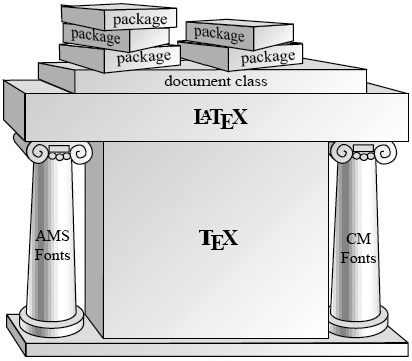
\includegraphics[width=8cm]{TexStone.png}\\
  \caption{\LaTeX{}\index{\LaTeX} 的结构示意图}{The structure of \LaTeX}
  \label{fig:TheStructureOfLaTeX}
\end{figure}


\TeX{}\index{\TeX} 是 \LaTeX{}\index{\LaTeX} 的基石, \LaTeX{}\index{\LaTeX} 建立在 \TeX{}\index{\TeX} 之上; 各种宏包和类型文件是 \LaTeX{}\index{\LaTeX}
大厦的装饰材料. \LaTeX{}\index{\LaTeX} 是特殊版本的 \TeX\index{\TeX}.

尽管在排版数学公式和数学符号方面, \LaTeX{}\index{\LaTeX} 不如 AMS\TeX, 但是 \LaTeX{}\index{\LaTeX} 提供了大量
易于学习和使用的命令, 例如非常有用的交叉引用命令等, 都是 AMS\TeX 所不具备的. 因而,
\LaTeX{}\index{\LaTeX} 的用途更为广泛, 特别是在排版信件、书刊、诗集等方面更优于 AMS\TeX.

自从 \LaTeX{}\index{\LaTeX} 问世以来, 流传最广的版本是 \LaTeX{}2.09\index{\LaTeX}. 由于 \LaTeX{}\index{\LaTeX} 的众多优点,
在计算机科学、数学及相关学科得到迅速广泛地应用, 吸引了许多专家、爱好者并为其编写和
添加了各式各样的宏包和宏库, 例如 PostScript 字体处理、排版复杂数学公式的 AMS\LaTeX{} 等,
这使得 \LaTeX{}\index{\LaTeX} 的功能不断地扩充, 应用领域不断地扩大. 但是, 由于没有统一的宏包编写
规划和编写格式, 造成某些宏包的功能彼此接近, 而命令相互冲突, 同一个源文件在某种格式
的 \LaTeX{}\index{\LaTeX} 中能够完美运行, 而在另一种格式中就可能编译出错或结果有所不同. 很多网站
和编辑部为了处理不同来源的 \LaTeX{}\index{\LaTeX} 文件, 不得不置备各种格式的 \LaTeX{}\index{\LaTeX} 系统; 有些
宏包很难分辨出是为那种格式编写的, 还得反复尝试.

有鉴于此, TUG 专门成立了 \LaTeX{}3\index{\LaTeX} 项目小组, 负责研发一个用途更加广泛, 功能更为完
善, 用户更易使用的崭新版本: \LaTeX{}3\index{\LaTeX}. 这是一个长期艰巨的科研计划, 为了尽快扭转当
时的混乱局面, \LaTeX{}3\index{\LaTeX} 项目小组先在 1994 年推出过渡版本 \LaTeX{}2$\varepsilon$\index{\LaTeX}.
新旧版本最明显的区别在于源文件的第一条命令, \LaTeX{}2.09 \index{\LaTeX} 为:
\begin{verbatim}
  \documentstyle[选项, 宏包名]{文件类型名}
\end{verbatim}
方括号里两种个不同类型的选择项并存, 容易产生混淆; \LaTeX{}2$\varepsilon$ \index{\LaTeX} 将其一分为二:
\begin{verbatim}
  \documentclass[选项]{文件类型名}
  \usepackage{宏包名}
\end{verbatim}
而且宏包也可以有自己的选项.

字体处理是新版最重要的改进, 它将 NFSS 作为标准的字体选择方法, 可处理任意编码的字体,
而旧版仅支持 OT1 编码. NFSS 是用属性的方式描述字体, 因此可分别独立地选择字体的某种
属性, 例如先选黑体, 再选斜体, 从而得到黑斜体, 这在旧版本是不可能的事儿.

新版本把 SLiTeX、AMSLaTeX 等宏库都归为附属的扩展宏包套件, 并将其中所有宏包的命令格
式统一, 可以用命令调用; 它还对浮动体定位、命令语句功能等方面进行了改进或扩充, 并对
旧版本中的错误和漏洞作了修补. 新版本还增添了许多新的功能、命令和错误提示信息以及处
理多种文字的 babel 宏包套件、图形制作的 graphics 宏包套件等.

新版本的另一个重要改进就是提供了更为高效便捷的宏包文件或类型文件编写命令.

新版本兼容旧版本, 也就是说用 \LaTeX{}2.09 \index{\LaTeX} 创建的源文件仍可在 \LaTeX{}2$\varepsilon$ \index{\LaTeX}
中运行, 只是速度要慢一半, 因为要在两种模式中切换; 如想要加快并享受新版的乐趣, 须将
源文件第一条命令改为新版形式.

\begin{figure}
  \centering
  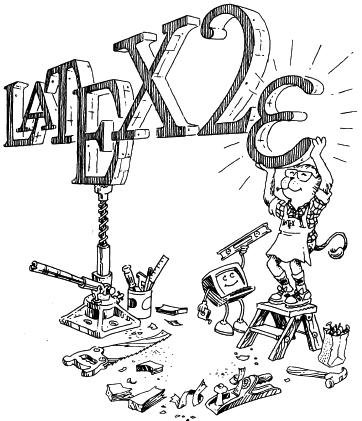
\includegraphics[width=8cm]{LaTeX2e.png}\\
\end{figure}

\LaTeX{} \index{\LaTeX}的读法应为``lay-teck", 念成``lay-tecks"也可以.

\LaTeX{}2$\varepsilon$ \index{\LaTeX}可读作``Lay-teck two e".

\LaTeX{} \index{\LaTeX}的标准写法比它的读法更别致, 应该是上图中的样子, 这在 \LaTeX{}\index{\LaTeX} 源文件中使用
专有命令就可轻易做到, 而在网页上很难实现, 为了简便起见, 都采用目前这种非常规大写形
式, \LaTeX{}2$\varepsilon$ \index{\LaTeX}也被简化成 \LaTeX{}2$\mathrm{e}$\index{\LaTeX}.

在 \LaTeX{}3 \index{\LaTeX}最终完成之前, \LaTeX{}2$\mathrm{e}$ \index{\LaTeX}仍将是标准的 \LaTeX{}\index{\LaTeX} 版本, 由
\LaTeX{}3 \index{\LaTeX}项目小组负责维护.

更多关于 \LaTeX{} \index{\LaTeX}的资料可以参考
\citet*{OetikerPartlHynaSchlegl2007,Leslie1994,MittelbachGoossensBraamsCarlisleRowley2004,ChenZhiJie2006,HuWei2011}.


\chapter{\LaTeX{} 与 Word 比较}{Compare \LaTeX with Word}
\LaTeX{}\index{\LaTeX} 与 Word 是两种不同类型的文本编辑处理系统, 各有所长, 如果要对文字编辑性能
和使用便捷程度等作综合评比, Word 明显优于 \LaTeX\index{\LaTeX}, 仅``所见即所得"一项, Word 就会
赢得绝大多数用户, 但要仅限定在学术报告和科技论文方面, 评比结果就不同了.

\section{从头开始}{From the Beginning}

Word 特点就是``所见即所得", 其基本功能初学者很容易掌握, 很多 Word 用户都是无师自
通. 但随着篇幅和复杂程度的增加, 花费在文稿格式上的精力和时间要明显加大, 如图
\ref{fig:CompareWithWord} 蓝
色示意曲线所示. 因为创建自定义编号、交叉引用、索引和参考文献等就不是``所见即所得"
了, 得耐着性子反复查阅 Word 的在线帮助或借助相关软件帮忙.

对于 \LaTeX{}\index{\LaTeX} 初学者, 即就是编排很简单的文章, 也要花较多的精力和时间去学习那些
枯燥的命令和语法, 特别是排写数学公式, 经常出错, 多次编译不能通过, 使很多初学者望
而却步. 可是一旦掌握, 不论文稿长短和复杂与否都会熟练迅速地完成, 先前学习 \LaTeX{}\index{\LaTeX}
的精力投入将由此得到回报, 如图 \ref{fig:CompareWithWord} 红色示意曲线所示.

\begin{figure}
  \centering
  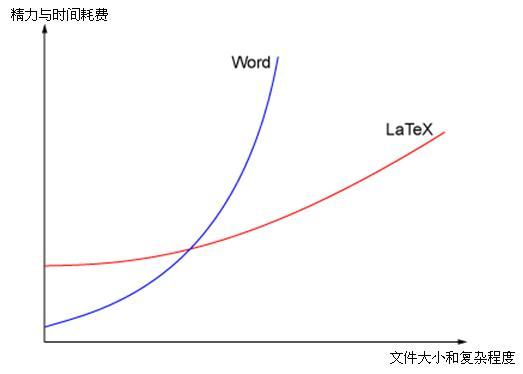
\includegraphics[width=9cm]{CompareWithWord.jpg}\\
  \caption{与 Word 比较}{Compare with Word}\label{fig:CompareWithWord}
\end{figure}

\section{内容与样式}{Contents and Format}
当用 Word 写作时, 要花很多精力对页版式、章节样式、字体属性、对齐和行距等文本参数进
行反复选择对比, 尤其是长篇文章, 经常出现因疏忽而前后文体格式不一致的现象; 当在稿件
中插入或删除一章或章节次序调整时, 各章节标题、图表和公式等的编号都要用手工作相应修
改, 稍有不慎就会出现重号或跳号. 你既是作者又是编辑还兼排字工.

使用 \LaTeX{}\index{\LaTeX} 编版, 如无特殊要求, 只要将文稿的类型 (article, report 或 book 等) 告
诉 \LaTeX\index{\LaTeX}, 就可专心致志地写文章了, 至于文稿样式的各种细节都由 \LaTeX{}\index{\LaTeX} 统一规划设
置, 而且非常周到细致; 当修改稿件时, 其中的章节、图表和公式等的位置都可任意调整, 无
须考虑编号, 因为在源文件里就没有编号, 文件中的所有编号都是在最后编译时 \LaTeX{}\index{\LaTeX} 自
动统一添加的, 所以绝对不会出错.

换句话说, Word 把文稿的内容与样式混为一体, 而 \LaTeX{}\index{\LaTeX} 将它们分离, 作者只需专注于
文稿的内容, 而文稿的样式几乎不用过问, \LaTeX{}\index{\LaTeX} 是你的聪明而忠诚的文字秘书, 如有特
殊要求, 也可使用命令修改, \LaTeX{}\index{\LaTeX} 会自动将相关设置更新, 无一遗漏.

接受 \LaTeX{}\index{\LaTeX} 稿件的出版社大都有自己的文稿样式模板, 主要就是一个类型文件包, 简称类
包. 如果稿件未被甲出版社采用, 在转投乙出版社前, 只需将稿件第一句中类包名称由甲出版
社的改为乙出版社的, 整篇稿件的样式就随之自动转换过来了. 就一句话的事儿, 简单的不能
再简单了, 然而因为``体制"的原故, Word 却根本无法做到这一点.

\section{数学公式}{Mathematical Formulas}
Word 有个公式编辑器, 可以编辑普通数学公式, 但使用很不方便, 外观效果较差, 也不能自
动编号, 尤其是很难作为文本的一部分, 融入某一行中, 大都专起一行. 如果碰到复杂的数学
公式, 编辑起来就很困难. 有些用户只好另外安装可嵌入 Word 环境的工具软件 MathType 来
弥补这一不足.

\LaTeX{}\index{\LaTeX} 的特长之一就是数学公式编辑, 方法简单直观, ``所想即所得", 公式的外观精致细
腻, 而且公式越复杂这一优点就越明显. 普通单行公式可以像纯文字文本一样插入字里行间.
下面举三例加以比较 (如图 \ref{fig:CompareTheDisplayOfWordAndLaTeX}), 其中 Word 分两
种情况, 一是 DOC 格式的屏幕显示效果, 二是将 DOC 格式文件通过 Acrobat 转换为 PDF 格
式的效果.

\begin{figure}
  \centering
  \begin{tabu}to.7\linewidth{X[1rm]X[1.5lm]}
    Word: & 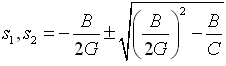
\includegraphics[width=5cm]{WordFormula.png}\\
    Word 转化为 PDF: & 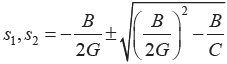
\includegraphics[width=5cm]{WordFormulaInPDF.png}\\
    \LaTeX{}: & $s_1$, $\displaystyle s_2=-\frac{B}{2G}\pm\sqrt{\left(\frac{B}{2G}\right)^2-\frac{B}{C}}$\\
  \end{tabu}
  \caption{Word 与 \LaTeX{}\index{\LaTeX} 公式显示效果对比}{Compare the display of Word and \LaTeX}
  \label{fig:CompareTheDisplayOfWordAndLaTeX}
\end{figure}

Word 在某些时候公式会出现对接不齐, 行距变宽等现象, 而 \LaTeX{}\index{\LaTeX} 编辑的公式在整个文档
中一直对接工整, 行距不变, 如图 \ref{fig:CompareTheAlignOfWordAndLaTeX}.

\begin{figure}
 \centering
 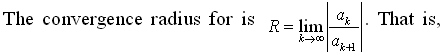
\includegraphics[width=9cm]{WordFormulaNotAlign.png}\\
 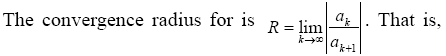
\includegraphics[width=9cm]{WordFormulaNotAlignInPDF.png}\\
 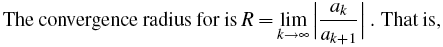
\includegraphics[width=9cm]{LatexFormulaAlign.png}\\
 \caption{Word 与 \LaTeX{}\index{\LaTeX} 公式的对齐比较}{Compare the align of Word and \LaTeX{}}
 \label{fig:CompareTheAlignOfWordAndLaTeX}
\end{figure}

尽管在默认状态下, 就能将数学公式编排的非常精致美观, \LaTeX{}\index{\LaTeX} 仍然还提供了很多调节
命令, 可以对公式的外观作更加细微的调整, 使其尽善尽美.

\section{插图}{Figures}

Word 有个绘图工具, 简易直观, 但功能有限效果不佳. 论文中的复杂图形大都用功能强大的
Visio、Photoshop 等绘图软件绘制, 然后插入 Word.

\LaTeX{}\index{\LaTeX} 自身也具有简单的绘图功能, 如调用各种绘图宏包, 可画出非常复杂的图形, 缺点
是不直观, 命令格式繁琐, 不易熟练掌握, 名曰画图, 实为编程. 可同样先使用 Visio 绘图,
然后粘贴到 Adobe Illustrator, 对图形的细节作进一步处理后, 存储为 PDF 或 EPS 格式,
最后用插图命令调入 \LaTeX{}\index{\LaTeX} 源文件即可, 其效果更为精致.

\section{创建参考文献}{Management References}

Word 目前还不具备管理参考文献的功能, 用户一般都是采用 Reference Manager 或是
NoteExpress 等外部工具软件来解决这一问题.

创建参考文献可是 \LaTeX{}\index{\LaTeX} 的强项. \LaTeX{}\index{\LaTeX} 自带一个辅助程序 BibTeX, 它可以根据作者
的检索要求, 搜索一个或多个文献数据库, 然后自动为文稿创建所需的参考文献条目列表. 如
果编写其它文件用到相同的参考文献时可直接引用这个数据库. 参考文献的样式和排序方式都
可以自行设定.

很多著名的科技刊物出版社、学术组织和 TUG 网站等都提供相关的 BibTeX 文献数据库文件,
可免费下载.

\section{显示与输出}{Display and Output}

在文本对齐、字体变换、拼写检查、单词间距控制、自动断词和自动换行等纯文字处理功能方
面, Word 经多次升版后已与 \LaTeX{}\index{\LaTeX} 相差无几, 但是排版效果却有所不同. 以 Times 字体
为例, 在 Word 中``Ta"和``PA"两个字母的间距有些松散, 见下图所示. \LaTeX{}\index{\LaTeX} 将各种拼写
组合时的字母间距进一步优化调整, 松紧得当, 使整个文本的排版效果更加工整匀称.

\begin{figure}
  \centering
  \begin{tabu}spread 1mm{X[-1rm]X[lm]}
    Word:\par\LaTeX: & 
\includegraphics[width=4cm]{WordPanda.pdf}\\
  \end{tabu}\vskip-5pt
\end{figure}

在换行时, \LaTeX{}\index{\LaTeX} 不仅可以根据音节自动断词, 也可以按照作者的要求进行设定断词, 一
个单词可以设定多种断词方式, 特别适用于科技论文中反复出现的专业词汇或缩略写, 这既能
保持单词间距均匀, 又不易产生误解.

在科技著作手稿中经常可以看到某些论述附有说明、出处或考证; 或者某些段落划上黑杠以示
删除; 或在边空里写有准备补充的文字. 在 \LaTeX{}\index{\LaTeX} 源文件中使用注释标记可以将上述这些
内容完整地保留下来, 以备后用, 而在编译后的 PDF 文件中还看不到这些内容. 科研论文要
经过反复推敲, 多次修改, 注释功能非常实用. ``所见即所得"的 Word, 当然没有这个功能,
它删除的内容就甭想再找回来了.

一篇论文, Word 新手与牛人的排版美观程度差别很大, ``所见即所得"成了一大缺点, 因为
Word 本身不能帮助作者美化作品, 自己排成什么样就什么样, 即: ``所得仅所见", 就像在白
纸上作画, 全凭个人的悟性与灵感. 而 \LaTeX{}\index{\LaTeX} 初学与专家的排版外观差别很小, 仅是快慢
不同, 都能达到专业出版水平, 这就是 \LaTeX{}\index{\LaTeX} 的一大优点, 只要想法一致就能得到相同的
结果, 即``所想即所得".

目前 PDF 格式已成为全世界各种组织机构用来进行更加安全可靠的电子文件分发和交换的出版
规范, 科技论文大都使用 PDF 格式. \LaTeX{}\index{\LaTeX} 可以直接输出 PDF、PS 或 DVI 格式文件; 而
Word 输出的是 DOC 格式文件, 还须购买 Adobe Acrobat 软件, 将 DOC 转换为PDF; 另外, 图
形中的数学公式或文本中数学式的上下标, 在转换后常出现位置偏移字形变大等问题.

\section{可扩充性}{Expansible}

用户可以像搭积木那样对 \LaTeX{}\index{\LaTeX} 进行功能扩充或添加新的功能. 例如, 加载一个 CJK 宏
包, 就可以处理中文, 调用 eucal 宏包可将数学公式中的字符改为欧拉书写体; 如果对某个
宏包效果不太满意, 完全可以打开来修改, 甚至照葫芦画瓢自己写一个. 这些可附加的宏包
文件绝大多数都可从 CTAN 等网站无偿下载.

因为设计的超前性, \TeX/\LaTeX{}\index{\LaTeX} 程序系统几十年来没有什么改动, 而且由于它的可扩充性,
\LaTeX{}\index{\LaTeX} 将永葆其先进性, 也就是说, 学习和使用 \LaTeX{}\index{\LaTeX} 永远不会过时. 例如, 通过调用
相关扩展宏包, \LaTeX{}\index{\LaTeX} 立刻就具备了排版高质量高专业水准象棋谱、五线谱或化学分子式
的能力. 对于 \LaTeX{}\index{\LaTeX} 这种机动灵活、简便免费的可扩充性能, Word 只能望尘.


\chapter{\LaTeX{}\index{\LaTeX} 应用情况}{The Application of \LaTeX}
我国已经有很多学术机构和高校校园网安装有 \TeX{}\index{\TeX} 或 \LaTeX{}\index{\LaTeX} 系统, 很多大专院校的教
师和学生、研究院所的科研人员以及出版社的编辑在使用 \LaTeX\index{\LaTeX}, 一些学术刊物开始接受使用
\LaTeX{}\index{\LaTeX} 排版的稿件。例如:《化学物理学报》已使用 C\TeX{} 排版英文期刊, 并鼓励作者
用 \LaTeX{}\index{\LaTeX} 排版投稿; 《计算数学》,《高能物理与核物理》,《电子与信息学报》,《应用数
学学报》等期刊的编辑部都要求作者提供 \LaTeX{}\index{\LaTeX} 源文件;《数学学报》和《工程数学学报》
更是明确指出定稿后作者必须提供 \LaTeX{}\index{\LaTeX} 源文件.

目前世界上许多权威学术机构都将 \LaTeX{}\index{\LaTeX} 排版格式作为标准的投稿文档格式. 例如: 国际
电子电气工程师协会, 美国工业和应用数学学会的各种期刊以及相关国际会议的论文都是将
\LaTeX{}\index{\LaTeX} 稿件列为首选; 美国数学学会将它所有出版物的稿件都要求用 \LaTeX{}\index{\LaTeX} 排版, 并提
供各种刊物的样式模板文件.

\LaTeX{}\index{\LaTeX} 作为一种专业的高品质排版系统, 已成为目前国际学术界最流行的排版系统, 很多
国际著名的出版机构都推荐或要求使用 \LaTeX\index{\LaTeX}. 例如: 荷兰爱思唯尔公司, 是世界著名的高
水准学术期刊出版商, 它出版的 1600 多种学术期刊中, 大部分都接受 \LaTeX{}\index{\LaTeX} 稿件, 有些
关于计算机、数学等方面的期刊还规定必须使用 \LaTeX{}\index{\LaTeX} 排版稿件, 并提供相应的 \LaTeX{}\index{\LaTeX}
样式模板和参考文献样式文件等; 德国施普林格公司是世界上著名的科技出版集团, 发行电子
图书并提供学术期刊检索服务, 目前共出版有 500 多种刊物, 其中大部分都可用 \LaTeX{}\index{\LaTeX} 投稿.
还有 Addison-Wesley, 牛津大学出版社等世界一流的出版社也都采用 \LaTeX{}\index{\LaTeX} 系统出版书籍
和期刊.
 
现在, 很多大型高科技企业也开始用 \LaTeX{}\index{\LaTeX} 排版订货合同、产品说明等, 因为有些商务文
件包含大量图形表格、数据指标、技术要求和相关标准引用, 其复杂和精细程度不亚于科技论
文.

毕竟 \LaTeX{}\index{\LaTeX} 是赠送给科技人员的写作工具, 它主要还是应用在科研报告和学术论文的排版,
用户大都是科研机构的研究人员和大专院校的师生. 虽然 \LaTeX{}\index{\LaTeX} 不是一天就能掌握的排版
系统, 但是一旦开始使用就会被它无穷的魅力所吸引. 随着科技的进步、网络时代的到来,
一定会有越来越多的科研工作者喜欢上 \LaTeX\index{\LaTeX}.

实际上, \LaTeX{}\index{\LaTeX} 已经逐渐成为科技文件发行和交流的主流出版标准.

\chapter{牛人简历}{Resumes of Supermans}
\label{cha:ResumesOfSupermans}
\section{Knuth 教授简历}{Resume of Pro. Knuth}

1938 年 12 月 7 日, Donald E. Knuth 出生于美国威斯康星州密尔沃基市. 其父是个中学教
师, 经常在星期天到教堂演奏管风琴, 小 Knuth 耳濡目染, 日后也成为教师, 业余爱好也是
弹管风琴.

\begin{figure}
  \centering
  \begin{minipage}[t]{0.3\textwidth}
    \centering
    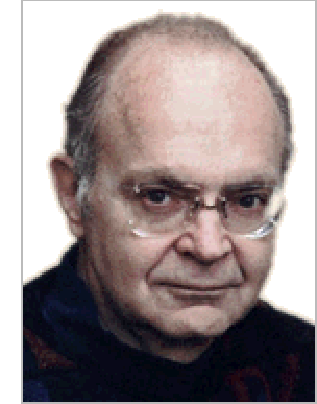
\includegraphics[width=3cm]{KnuthPhoto.pdf}
    \caption{Knuth 教授头像}{The head portrait of Pro. Knuth}
  \end{minipage}
  \hspace{1cm}
  \begin{minipage}[t]{0.3\textwidth}
    \centering
    \includegraphics[width=3.8cm]{knuthPhotoCartoon.pdf}
    \caption{Knuth 教授卡通头像}{The cartoon portrait of Pro. Knuth}
  \end{minipage}
\end{figure}


1956 年进入俄亥俄州克利夫兰的凯斯理工学院 (现并入凯斯西储大学), 学习物理.

1957 年大学一年级暑假在学校打工, 接触到当时很先进的 IBM650 计算机, 产生浓厚兴趣.

1958 年改学数学, 并从此与计算机结缘.

1960 年毕业, 因为成绩过于出色, 校方打破惯例, Knuth 被同时授予学士和硕士学位. 随后
进入加州理工学院数学系.

1960 -- 1968 年, 兼任 Burroughs 公司顾问.

1961 年结婚, 夫人小他一岁. 现有一儿一女.

1963 年取得博士学位, 并留校任助理教授.

1964 -- 1967年, 兼任美国计算机协会刊物《程序设计语言》编辑.

1966 年升为副教授.

1968 年任教于斯坦福大学计算机科学系, 正教授. 同年, 开始撰写著名的《计算机程序设计
艺术》一书.

1968 年《计算机程序设计艺术》第一卷《基本算法》出版.
1969 年, 第二卷《半数字化算法》出版.
1971 年获首届美国计算机协会格蕾丝 $\cdot$ 赫柏奖.
1973 年, 第三卷《排序与搜索》出版. 同年还出版了第一卷的第二版. 有人曾说, 看了这部
书后, 再谈起编程序都会变得谦虚谨慎. 比尔 $\cdot$ 盖茨曾说:``如果你能读懂整套书的
话,请给我发一份你的简历."同年, 当选为美国科学艺术学院院士. 截至到 1973 年的第一卷
第二版, 采用都是的活字排版印刷, 这需要经验丰富的活字排版工人.

1974 年, 因在算法分析和编程语言设计方面的突出贡献, 荣获美国计算机协会图灵奖, 是历
史上最年轻的获奖者. 图灵奖被称为计算机界的诺贝尔奖. 《计算机程序设计艺术》一书与
牛顿的《自然哲学的数学原理》等书一起, 被评为``世界历史上最伟大的十种科学著作"之一.

1975 年当选为美国国家科学院院士.

1976 年出版第二卷第二版时采用了计算机排版技术. 但是, 当时的计算机排版与活字排版效
果相差甚远, 而且前后两卷的字体、版式和文本格式等都不一致. 非常失望的 Knuth 暂停了
第二卷第二版的出版, 决心自己设计一个比活字排版更加优美和适用的排版软件, 这就是后来
的 \TeX.

1977 年 5 月开始构造后来被称为 \TeX{} 的文字处理系统, 他研究了古今的排版技术, 把其
中最优越的部分引入 \TeX{} 中, 连 \TeX{} 中的字体 (METAFONT) 全部都是他自行设计的.
同年, 访问中国三周, 行前姚储枫给他起了个中文名字: 高德纳. (姚储枫, 姚期智的夫人,
夫妇都是著名计算机科学家, 2000 年姚期智获图灵奖.)

1978 年应邀在美国数学学会年会上作报告, 题为``数学排版 --- \TeX{} 与 METAFONT",引起
数学界关注.

1979 年, Knuth 教授的著作《\TeX{} 与 METAFONT: 排版的新趋势》, 由数字设备公司和美
国数学学会联合出版. 同年, 荣获美国总统卡特授予的科学金奖.

1980 年获国际电子电气工程师协会计算机学会麦可道尔奖. 同年, 成为英国计算机学会会员.

1981 年当选为美国工程院院士.

1982 年使用自己设计的 \TeX{} 软件和字体, Knuth 如愿出版了《计算机程序设计艺术》的第
二卷第二版. 之后, Knuth 还不遗余力地改进 \TeX, 并在 \TeX{} 的稳定性上下了很大功夫.
在基本式样没有改变的情况下, \TeX{} 第 3 版又追加了很多功能. 9 月, 公布了 DVI 驱动
程序. 同年, 成为国际电子电气工程师协会荣誉会员, 并获计算机先锋奖.

1984 年, 艾迪生---韦斯利公司出版 Knuth 教授的《The TeXbook》, 该书成为最权威的 \TeX{}
参考书.

1985 年, 将 \TeX{} 的默认字体由美国现代改为计算机现代.

1986 年荣获美国数学学会的斯蒂尔奖.

1987 年获纽约科学研究会奖.

1988 年获富兰克林奖.

1989 年, 因其对软件理论的贡献获 J.D. Warnier 奖.

1990 年, 斯坦福大学授予他计算机科学艺术教授的称号.

1991 年, 《3:16 圣经文本阐释》一书出版, 他试图用分层随机抽样的方法对圣经进行分析.

1992 年退休, 但还是斯坦福大学和牛津大学的客座教授. 他这么早退休的原因, 就是因为研究
开发 \TeX{} 系统延误了编写出版《计算机程序设计技巧》这部书, 他估计还要花 20 年来完
成. 目前此书前三卷已出版, 预计要出到第七卷.

1993 年宣布不再对 \TeX{} 和 METAFONT 进行更新.

1994 年获瑞典皇家科学院克努特奖.

1995 年获国际电子电气工程师协会的纽曼奖和以色列的科学与艺术哈维奖.

1996 年 11 月, 由于发明先进的排版技术荣获京都先进技术奖 (日本最高终身成就奖, 奖金
约 46 万美元, 被称为日本的诺贝尔奖).

1997 年对《计算机程序设计技巧》前三卷作了修订.

2001 年国际天文学联合会把两年前发现的第 21656 号小行星命名为``Knuth".

2003 年荣获马其顿大学荣誉博士, 同年当选英国皇家学会的外籍院士.

2004 年《计算机程序设计技巧》前三卷再版发行.

\begin{figure}
  \centering
  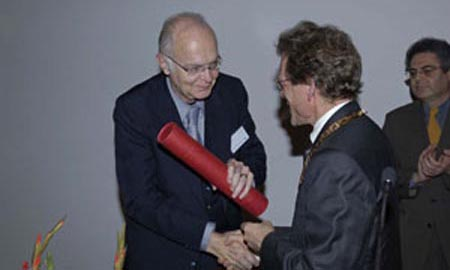
\includegraphics[width=9cm]{Knuth2005.jpg}\\
\end{figure}

2005 年 11 月, 从瑞士联邦苏黎士高等理工学院院长手中接过荣誉博士证书.

现在, 正在编写《计算机程序设计技巧》其余几卷.
 
他的所有著作都有个奇特``附加效应", 那就是任何人发现书中的错误, 不论是技术上的或是
排版上的还是历史上的错误, 都可以向他指出, 并可领取 2.56 美元! 可见其人幽默诙谐而且
能够闻过则喜.

\begin{figure}
  \centering
  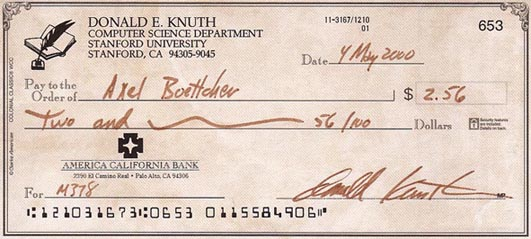
\includegraphics[width=10cm]{KnuthCheck.jpg}\\
  \caption{Knuth 教授的支票}{The check of Pro. Knuth}
\end{figure}


为什么是 2.56 美元? Knuth 教授的答案是:``256 pennies is one hexadecimal dollar."
 
从 1981 年夏至 1996 年 7 月 1 日, Knuth 教授给指出错误的人回信 250 多封, 其中一半
以上装有奖励支票. 从奖励支票清单来看, 有一位名叫 Axel B\"{o}ttcher  的人, 曾先后 5
次得到两块五毛六的支票, 3 次得到五块一毛二的支票, 真可谓牛人背后有牛人.
 
受麦粒与棋盘的故事影响, Knuth 教授宣布, 每发现一个 \TeX{} 程序或 METAFONT 程序中的
错误, 奖励从 2.56 美元开始, 每年翻倍, 最高为 327.68 美元. 1995 年有两人领取了这项
奖金, 此后至今, 还无人能够认领!
 
有网友戏说, 什么是聪明: 在 Knuth 的书中找到错误; 什么是愚蠢: 去兑现那张两块五毛六的
支票.
 
Knuth 教授是法国、挪威和德国科学院的外籍院士; 还是牛津大学、巴黎大学、斯德哥尔摩皇
家理工学院、奥斯陆大学、安特卫普大学、圣彼得堡大学和马其顿大学等十几所大学的荣誉博士.

Knuth 教授带过 28 个研究生, 拥有 5 项专利, 出版 25 部著作, 发表 160 篇论文; 他的著
作已有 6 种文字译本, 发行量超过一百万册. 英文版的《计算机程序设计艺术》一书已再版
11 次, 该书前三卷中文版于 1978 年至 1992 年陆续出版, 由苏运霖教授翻译, 他曾在 1977
年与来访的 Knuth 教授在北京座谈.

Knuth 教授爱好音乐, 年轻时曾考虑报考音乐专业. 在他的书房中放了一个特别定制的 84 管
的管风琴. 他还会吹萨克斯管和大号.
            
\TeX{} 是二十世纪排版技术方面最重大的发明, 历经 20 年的岁月, \TeX{} 在基本没有改动
的情况下被世界各地各种语言的人们广泛使用, \TeX{} 的优美排版效果令使用者爱不释手.
现在, 世界上很多国家都有 \TeX{} 用户组织, \TeX{} 不断地被推广和扩展.

Knuth 教授因在 \TeX{} 及计算机编程方面的巨大贡献和他大量创造性的影响深远的著作而享
誉全球.

Donald E. Knuth 这个名字将和 \TeX{} 一起被载入世界科学史册.

\section{Lamport 博士简历}{Resume of Pro.Lamport}

\begin{figure}
  \centering
  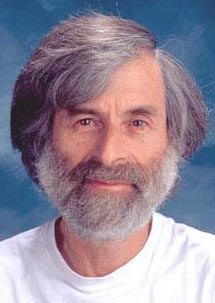
\includegraphics[width=4cm]{LeslieLamport.jpg}\\
  \caption{Lamport 教授的头像}{The head portrait of Pro. Lamport}
\end{figure}

1941 年 Leslie Lamport 生于纽约.

1960 年毕业于麻省理工学院数学专业.

1963 年获得布兰迪斯大学数学硕士学位.

1965 -- 1969 年任教于马尔波罗学院.

1970 -- 1972 年, 麻省计算机协会系统设计员.

1972 年获得布兰迪斯大学数学博士学位.

1972 -- 1977 年, 麻省计算机协会研究员.

1977 -- 1985 年, SRI 公司计算机科学实验室任究员.

1982 年与另两人共同发表论文``拜占廷将军问题", 既允许军中可能有叛徒, 又要保证战争胜
利, 引申到计算机领域, 成为一种容错理论.

1984 年前后, 使用 Knuth 教授发明的 Plain \TeX{} 排版软件撰写一些并行计算方面的论文,
感到还是不太方便, 于是编写了便于自己使用的宏包套件, 并命名为 \LaTeX. 其主要改进是将
版面设计与文稿内容分开处理, 只要使用者选择了一种文件类别, \LaTeX{} 自动将整本书或整
篇文章的结构和标题就按照这种文件类別典型样式来设置, 作者只要专注文章的內容就可以了.
起初 \LaTeX{} 在计算机科学家之间流传, 大家觉得 \LaTeX{} 比 Plain \TeX{} 使用更方便,
就经常通过各种渠道向他索取.

1984 年发表论文``分布系统中的时间、时钟和事件排序".

1985 -- 2001 年, 在数字设备公司以及康柏系统研究中心作研究工作. (1998年, 康柏计算机
公司收购了数字设备公司. 2002 年惠普公司完成收购康柏公司之后, 数字设备公司的剩余部分
并入了惠普公司. )

1985 年, 花两个月时间将 \LaTeX{} 源代码整理出来, 并编写出版了一本 \LaTeX{} 使用手册
《\LaTeX: 一种文稿排版系统》, 当时流行的 \LaTeX{} 版本为 2.09.

1989 年 8 月 21 日, 在斯坦福大学 \TeX{} 用户组织会议上, 同意将 \LaTeX{} 的维护和开
发工作交给 \LaTeX{}3 小组.

1994 年, 与 \LaTeX{}3 小组对 \LaTeX{} 作了一次重大改进, 版本命名为 \LaTeX{}2$\varepsilon$,
并出版 \LaTeX{} 使用手册第二版.

\begin{figure}
  \centering
  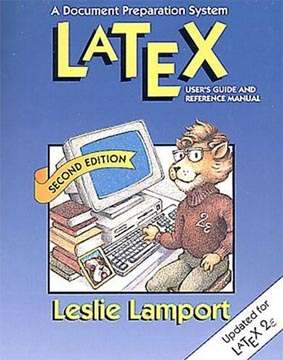
\includegraphics[width=6cm]{LaTeXADocumentPreparationSystem.jpg}\\
  \caption{\LaTeX: 一种文稿排版系统封面}{\LaTeX: A document preparation system}
\end{figure}


2001 年进入位于加利福尼亚的微软研究院, 任高级研究员, 从事分布式计算机系统理论研究.

2003 年获法国雷恩大学荣誉博士.

\begin{figure}
  \centering
  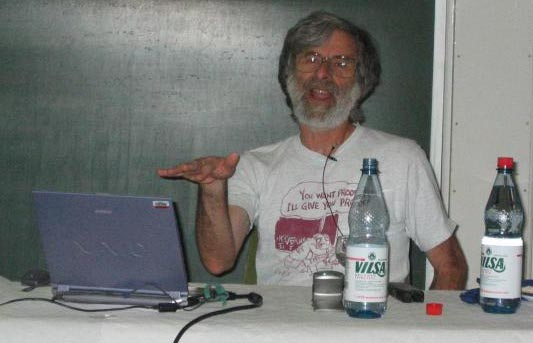
\includegraphics[width=8cm]{LamportYouWantProof.jpg}\\
  \caption{德国基尔大学作学术报告}{Lecture in Christian-Albrechts-Universit\"{a}t zu Kiel}
\end{figure}

2004 年, 由于在计算机信息处理方面的突出贡献, 获得皮奥尔奖. 同年获瑞士洛桑联邦工业
大学荣誉博士.

截至 2006 年, 已发表论文 160 篇.


\chapter{BSDE 的 $L^1$ 解的存在唯一性}{An existence and
uniqueness result for $L^1$ solutions of BSDEs}
\label{cha:FiniteTimeInterval}

在本节中, 我们考虑如下一维倒向随机微分方程:
\begin{equation}\label{eq:BSDEsInFiniteTimeInterval}
  y_t=\xi+\intT{t} g(s,y_s,z_s)\dif s-\intT{t} z_s\cdot\dif B_s,\quad t\in\tT,
\end{equation}
其中 $\xi$ 在 $\rtn$ 中取值; $T$ 有限, 即 $0\leq T<+\infty$; 生成元 $g$ 定义如下
$$g(\omega,t,y,z):\Omega\times\tT\times\rtn\times\rtn^d\mapsto \rtn,$$
且对任意的 $(y,z)\in\rtn\times\rtn^d$, $g(\cdot,\cdot,y,z)$ 为
$(\F_t)$-循序可测的随机函数. 即在本节中, 我们总假定 $k=1$.

\begin{definition}\label{def:DefinitionOfBSDEInFiniteTimeInterval}
  BSDE \eqref{eq:BSDEsInFiniteTimeInterval} 的解是指一对在空间 $\rtn\times\rtn^d$
  中取值的 $(\F_t)$-适应过程 $(y_t,z_t)_{t\in\tT}$, 它们满足 $\prs$, $t\mapsto y_t$
  连续, $t\mapsto z_t$ 属于空间 $L^2(0,T)$, $t\mapsto g(t,y_t,z_t)$ 属于空间 $L^1(0,T)$,
  并且 $\prs$, 对于任意的 $t\in\tT$, BSDE \eqref{eq:BSDEsInFiniteTimeInterval} 恒成立.
\end{definition}

\citet*{PardouxPeng1990SCL} 首先研究了这种方程的非线性形式, 并且在生成元 $g$ 满足
 Lipschitz 条件下建立了参数平方可积的多维 BSDE 的解的存在惟一性. 从此之后,
很多学者致力于减弱生成元 $g$ 的 Lipschitz 条件, 例如, \citet*{Mao1995SPA},
\cite*{LepeltierSanMartin1997SPL} 等. 众所周知, 求解参数仅仅可积的 BSDE 要比求解参
数平方可积的 BSDE 困难. 据我们所知, 仅有几篇文章研究了参数仅仅可积的 BSDE, 如
\citet*{BriandDelyonHu2003SPA}. 我们主要研究一类终端时
间 $T$ 有限且参数仅仅可积的一维 BSDEs 的 $L^1$ 解的存在惟一性, 其中生成元 $g$
关于 $y$ 是 Lipschitz 连续, 关于 $z$ 是 $\alpha$-H\"{o}lder 连续的, 其中
 $0<\alpha<1$. 此部分结果已发表在 Statistics and Probability Letters, 可见
 \citet*{FanLiu2010SPL}.

首先介绍需要用到的假设条件.

\begin{enumerate}
\renewcommand{\theenumi}{(B\arabic{enumi})}
\renewcommand{\labelenumi}{\theenumi}

  \item\label{HInFiniteTimeInterval:OnlyIntegrable}
          $\EX
          \left[|\xi|+
              \intT{0}|g(t,0,0)|\dif t
          \right]<+\infty$;
  \item\label{HInFiniteTimeInterval:LipschitzAndAlphaHolder}
       存在两个常数 $\mu$, $\alpha>0$ 满足 $\pts$, 对于任意的 $(y_i,z_i)\in\rtn\times\rtn^d$ $(i=1,2)$,
       \begin{equation*}
         |g(t,y_1,z_1)-g(t,y_2,z_2)|\leq \mu|y_1-y_2|+\mu|z_1-z_2|^\alpha.
       \end{equation*}
\end{enumerate}

\begin{remark}
  本节最主要的假设 \ref{HInFiniteTimeInterval:LipschitzAndAlphaHolder} 等价于下
  面的两个条件:
  \begin{enumerate}
    \renewcommand{\theenumi}{(H\arabic{enumi})}
    \renewcommand{\labelenumi}{\theenumi}

    \item $g$ 关于 $y$ 满足对 $(\omega,t,z)$ 一致的 Lipschitz 连续条件, 即存在一
          个常数 $\mu>0$ 使得 $\pts$,
          $$\forall y_1,y_2,z, \quad |g(t,y_1,z)-g(t,y_2,z)|\leq\mu|y_1-y_2|;$$
    \item $g$ 关于 $z$ 满足对 $(\omega,t,y)$ 一致的 H\"older 连续条件, 即存在两个
          常数 $\mu$, $\alpha>0$ 使得 $\pts$,
          $$\forall y,z_1,z_2,\quad |g(t,y,z_1)-g(t,y,z_2)|\leq\mu|z_1-z_2|^\alpha.$$
  \end{enumerate}
\end{remark}


下面的定理 \ref{thm:FiniteTimeIntervalL1Solution} 是本节的主要结果.

\begin{theorem}\label{thm:FiniteTimeIntervalL1Solution}
  假设 \ref{HInFiniteTimeInterval:OnlyIntegrable} 和 \ref{HInFiniteTimeInterval:LipschitzAndAlphaHolder}
  成立且 $\alpha\in(0,1)$, 则 BSDE \eqref{eq:BSDEsInFiniteTimeInterval} 存在惟一
  解 $(y_t,z_t)_{t\in\tT}$ 使得 $(y_t)_{t\in\tT}$ 属于 (D) 类, 且
  $(z_t)_{t\in\tT}$ 属于空间 $\bigcup_{\beta>\alpha}\Mm^\beta$. 进一步地, 对于任意的
  $\beta\in(0,1)$,
  $(y_t,z_t)_{t\in\tT}$ 属于空间 $\s^\beta\times\Mm^\beta$.
\end{theorem}

\begin{example}
  令 $g(t,y,z)=\sin y+\sqrt{|z|}+|B_t|$. 则由定理 \ref{thm:FiniteTimeIntervalL1Solution}
  可得, 对于任意的 $\xi\in L^1(\Omega,\F_T,\PR)$, BSDE \eqref{eq:BSDEsInFiniteTimeInterval}
  存在惟一解 $(y_t,z_t)_{t\in\tT}$ 使得 $(y_t)_{t\in\tT}$~
  属于 (D) 类且
   $(z_t)_{t\in\tT}$ 属于 $\bigcup_{\beta>1/2}\Mm^\beta$.
\end{example}

为介绍 \citet*{BriandDelyonHu2003SPA} 中的结果, 我们做如下假设:
  \begin{enumerate}
    \renewcommand{\theenumi}{(B\arabic{enumi}')}
    \renewcommand{\labelenumi}{\theenumi}
    \setcounter{enumi}{1}

%    \item \label{HBriandDelyon:OnlyIntegrable}
%          $\EX\left[|\xi|+\intT{0}|g(s,0,0)|\dif s\right]<+\infty$;
    \item \label{HBriandDelyon:gContinuousInY}
          $\pts$, 对于任意的 $z$, $y\mapsto g(\omega,t,y,z)$ 连续;
    \item \label{HBriandDelyon:gMonotonicInY}
          $g$ 关于 $y$ 单调, 即存在一个常数 $\mu\geq 0$ 使得 $\pts$,
          $$\forall y_1,y_2,z, \quad \big(g(t,y_1,z)-g(t,y_2,z)\big)(y_1-y_2)\leq \mu|y_1-y_2|^2;$$
    \item \label{HBriandDelyon:gGeneralGrowthInY}
          $g$ 关于 $y$ 满足一般增长条件, 即对于任意的 $r>0$, 有
          $$\varphi_r(t):=\sup_{|y|\leq r}|g(t,y,0)-g(t,0,0)|\in L^1(\tT\times\Omega);$$
    \item \label{HBriandDelyon:gLipschitzContinuousInZ}
          $g$ 关于 $z$ 是 Lipschitz 连续的, 且关于 $(\omega,t,y)$ 一致, 即存在
          常数 $\lambda\geq 0$ 使得 $\pts$,
          $$\forall y,z_1,z_2,\quad |g(t,y,z_1)-g(t,y,z_2)|\leq\lambda|z_1-z_2|;$$
    \item \label{HBriandDelyon:gSublinearGrowthInZ}
          存在两个常数 $\gamma\geq 0$, $\alpha\in(0,1)$ 和一个非负 $(\F_t)$-循序
          可测过程 $(g_t)_{t\in\tT}$ 且 $\EX[\intT{0}g_t\dif t]<+\infty$, 使得 $\pts$,
          $$\forall y,z, \quad |g(t,y,z)-g(t,y,0)|\leq \gamma(g_t+|y|+|z|)^\alpha.$$
  \end{enumerate}

下面的引理 \ref{lem:BriandDelyonL1Solution} 是 \citet*{BriandDelyonHu2003SPA} 中定理
 6.2 和定理 6.3 的一维版本.

\begin{lemma}\label{lem:BriandDelyonL1Solution}
  假设 \ref{HInFiniteTimeInterval:OnlyIntegrable}, \ref{HBriandDelyon:gContinuousInY} -- \ref{HBriandDelyon:gSublinearGrowthInZ}
  成立, 则 BSDE $(\xi,T,g)$ 存在惟一解 $(y_t,z_t)_{t\in\tT}$ 使得, $(y_t)_{t\in\tT}$
  属于 (D) 类且 $(z_t)_{t\in\tT}$ 属于 $\bigcup_{\beta>\alpha}\Mm^\beta$. 进一步地,
  对于任意的 $\beta\in(0,1)$, $(y_t,z_t)_{t\in\tT}$ 属于空间 $\s^\beta\times\Mm^\beta$.
\end{lemma}

下面我们开始证明定理 \ref{thm:FiniteTimeIntervalL1Solution}.

我们首先建立如下命题 \ref{pro:ComparisonTheoremInFiniteTimeInterval}, 定理
 \ref{thm:FiniteTimeIntervalL1Solution} 的惟一性部分是此命题的直接推论.

\begin{proposition}\label{pro:ComparisonTheoremInFiniteTimeInterval}
  假设生成元 $g$ 满足 \ref{HInFiniteTimeInterval:LipschitzAndAlphaHolder} 且
  $\alpha\in(0,1]$, 令 $(y_t,z_t)_{t\in\tT}$ 和 $(y'_t,z'_t)_{t\in\tT}$ 分别表示
   BSDE $(\xi,T,g)$ 和 BSDE $(\xi',T,g)$ 的解, 使得 $(y_t)_{t\in\tT}$ 和 $(y'_t)_{t\in\tT}$
  都属于 (D) 类, 且 $(z_t)_{t\in\tT}$ 和 $(z'_t)_{t\in\tT}$ 都属于
   $\bigcup_{\beta>\alpha}\Mm^\beta$. 如果 $\prs$, $\xi\leq\xi'$, 则对于任意的 $t\in\tT$,
  有
  $$\prs, \quad y_t\leq y'_t.$$
\end{proposition}

\begin{proof}
  此命题的证明借鉴于 \citet*{BriandDelyonHu2003SPA}. 我们先固定 $n\in\N$, 且令 $\tau_n$
  表示停时
  \begin{equation*}
    \tau_n=\inf\left\{t\in\tT:\int^t_0\left(|z_s|^2+|z'_s|^2\right)\dif s
    \geq n\right\}\wedge T.
  \end{equation*}
  令 $\hat{y}_t=y_t-y'_t$, $\hat{z}_t=z_t-z'_t$, 则对 $\me^{\mu t}\hat{y}_t$
  作用 Tanaka 公式可以得到
   \begin{align*}
     \me^{\mu(t\wedge\tau_n)}\hat{y}^+_{t\wedge\tau_n}
     \leq &\ \me^{\mu\tau_n}\hat{y}^+_{\tau_n}
       -\intT[\tau_n]{t\wedge\tau_n}\me^{\mu s}
        \one{\hat{y}_s>0}\hat{z}_s\cdot\dif B_s\nonumber\\
     &+\intT[\tau_n]{t\wedge\tau_n}\me^{\mu s}
        \left\{
          \one{\hat{y}_s>0}
          [g(s,y_s,z_s)-g(s,y'_s,z'_s)]-\mu\hat{y}^+_s
        \right\}\dif s.
   \end{align*}
  由假设 \ref{HInFiniteTimeInterval:LipschitzAndAlphaHolder} 可得,
  \begin{equation}\label{eq:TanakaResultInProofOfUniquenessFiniteTimeInterval}
    \me^{\mu(t\wedge\tau_n)}\hat{y}^+_{t\wedge\tau_n}
    \leq \me^{\mu\tau_n}\hat{y}^+_{\tau_n}
      +\intT[\tau_n]{t\wedge\tau_n}\mu\me^{\mu s}
         \one{\hat{y}_s>0}|\hat{z}_s|^\alpha\dif s
      -\intT[\tau_n]{t\wedge\tau_n}\me^{\mu s}
       \one{\hat{y}_s>0}\hat{z}_s\cdot\dif B_s.
  \end{equation}
  对上式左右两侧关于 $\F_t$ 取条件期望并注意到 $\tau_n\leq T$ 可得,
  \begin{equation*}
    \me^{\mu(t\wedge\tau_n)}\hat{y}^+_{t\wedge\tau_n}
    \leq \me^{\mu T}\EX
         \left[\left.
           \hat{y}^+_{\tau_n}
           +\mu\intT[\tau_n]{t\wedge\tau_n}|\hat{z}_s|^\alpha\dif s
           \right|\F_t
         \right]
    \leq \me^{\mu T}\EX
         \left[\left.
           \hat{y}^+_{\tau_n}
           +\mu\intT{0}|\hat{z}_s|^\alpha\dif s
           \right|\F_t
         \right].
  \end{equation*}
  下面我们先证明 $(\hat{y}^+_t)_{t\in\tT}\in\s$. 由于 $(y_t)_{t\in\tT}$ 和
   $(y'_t)_{t\in\tT}$ 都属于 (D) 类, $(\hat{z}_t)_{t\in\tT}\in\bigcup_{\beta>\alpha}\Mm^\beta$,
  并且考虑到 $\xi\leq\xi'$, 于是在上不等式中令 $n\to\infty$ 可得, 对于任意的 $t\in\tT$,
  \begin{equation*}
    \hat{y}^+_t\leq\mu\me^{\mu(T-t)}\EX
    \left[\left.
      \intT{0}|\hat{z}_s|^\alpha\dif s\right|\F_t
    \right],
  \end{equation*}
  然后根据 Jensen 不等式, Doob 不等式和 H\"older 不等式可得, 存在一个仅依赖于
   $\alpha$ 和 $\beta$ 的常数 $C$ 使得
  \begin{equation*}
    \EX
    \left[
      \sup_{t\in\tT}|\hat{y}^+_t|^{\beta/\alpha}
    \right]
    \leq C\EX
         \left[
           \left(
             \intT{0}|\hat{z}_s|^2\dif s
           \right)^{\beta/2}
         \right]<+\infty.
  \end{equation*}
  从而得出 $(\hat{y}^+_t)_{t\in\tT}\in\s$.

  下面我们介绍一个对后面的证明起到关键作用的不等式, 是关于函数
   $x^\alpha$ ($\alpha\in(0,1]$) 的一个简单估计:
  \begin{equation}\label{eq:SimpleEstimateOnXAlpha}
    \forall m\geq 1, x\in\rtn^+,\quad x^\alpha\leq mx+\frac{1}{m^\alpha}.
  \end{equation}
  事实上, 如果 $0\leq x\leq 1/m$, 由于 $x^\alpha\leq 1/m^\alpha$, 那么
   \eqref{eq:SimpleEstimateOnXAlpha} 显然成立. 如果 $1/m<x<1$, 那么 $mx>1>x^\alpha$.
  如果 $x\geq 1$, 仍然有 $mx\geq x\geq x^\alpha$.

  对于任意的 $m\geq 1$, 由 \eqref{eq:TanakaResultInProofOfUniquenessFiniteTimeInterval}
  和 \eqref{eq:SimpleEstimateOnXAlpha} 可得,
  \begin{align}\label{eq:GirsanovChangeInComparisonTheoremProof}
    \me^{\mu(t\wedge\tau_n)}\hat{y}^+_{t\wedge\tau_n}
    &\leq \me^{\mu\tau_n}\hat{y}^+_{\tau_n}
         +\intT[\tau_n]{t\wedge\tau_n}\mu\me^{\mu s}\one{\hat{y}_s>0}
          \left[
            m|\hat{z}_s|+\frac{1}{m^\alpha}
          \right]\dif s
         -\intT[\tau_n]{t\wedge\tau_n}\me^{\mu s}\one{\hat{y}_s>0}\hat{z}_s\cdot\dif B_s\nonumber\\
    &\leq \me^{\mu\tau_n}\hat{y}^+_{\tau_n}
          \!+\!T\me^{\mu T}\frac{\mu}{m^\alpha}
          -\!\intT[\tau_n]{t\wedge\tau_n}\!\!\!\me^{\mu s}\one{\hat{y}_s>0}\hat{z}_s\cdot\!
          \left[
            -\frac{m\mu\hat{z}_s}{|\hat{z}_s|}\one{|\hat{z}_s|\neq 0}\dif s+\!\dif B_s
          \right]\!.
  \end{align}
  令 $\PR_m$ 表示在概率空间 $(\Omega,\F)$ 中与 $\PR$ 等价的概率测度, 定义为
  \begin{equation*}
    \frac{\dif \PR_m}{\dif \PR}:=\exp
    \left\{
      m\mu\intT{0}\frac{\hat{z}_s}{|\hat{z}_s|}\one{|\hat{z}_s|\neq 0}\cdot\dif B_s
      -\frac{1}{2}m^2\mu^2\intT{0}\one{|\hat{z}_s|\neq 0}\dif s
    \right\}.
  \end{equation*}
  值得注意的是, $\dif\PR_m/\dif\PR$ 有任意阶矩. 由 Girsanov 定理, 在 $\PR_m$ 测
  度下, 随机过程
  $$B_m(t)=B_t-\intT[t]{0}\frac{m\mu\hat{z}_s}{|\hat{z}_s|}\one{|\hat{z}_s|\neq 0}\dif s, \quad t\in\tT$$
  是一个 $(\F_t,\PR_m)$-布朗运动. 此外, 随机过程
  $$\left(\intT[t\wedge\tau_n]{0}\me^{\mu s}\one{\hat{y}_s>0}\hat{z}_s\cdot\dif B_m(s)\right)_{0\leq t\leq T}$$
  是一个 $(\F_t,\PR_m)$-鞅. 令 $\EX_m[X|\F_t]$ 表示随机变量 $X$ 关于 $\F_t$
  在 $\PR_m$ 概率下的条件期望. 对~\eqref{eq:GirsanovChangeInComparisonTheoremProof}
  两侧关于 $\F_t$ 在 $\PR_m$ 概率下取条件期望, 可以得到, 对于任意的 $m\geq 1$, $t\in\tT$,
  \begin{equation}\label{eq:AfterGirsanovChangeInComparisonTheoremProof}
    \me^{\mu(t\wedge\tau_n)}\hat{y}^+_{t\wedge\tau_n}
    \leq \EX_m
         \left[\left.
           \me^{\mu\tau_n}\hat{y}^+_{\tau_n}\right|\F_t
         \right]
         +\frac{T\me^{\mu T}\mu}{m^\alpha}.
  \end{equation}

  最后, 既然 $(\hat{y}^+_t)_{t\in\tT}\in\s$, 并且考虑到 $\xi\leq\xi'$, 我们可以
  在 \eqref{eq:AfterGirsanovChangeInComparisonTheoremProof} 中令 $n\to\infty$,
  于是对于任意的 $m\geq 1$, $t\in\tT$,
  \begin{equation*}
    \me^{\mu t}\hat{y}^+_{t}\leq T\me^{\mu T}\frac{\mu}{m^\alpha},
  \end{equation*}
  因此通过令 $m\to\infty$ 可以得出命题 \ref{pro:ComparisonTheoremInFiniteTimeInterval}
  的结论.
\end{proof}

有了命题 \ref{pro:ComparisonTheoremInFiniteTimeInterval}, 定理 \ref{thm:FiniteTimeIntervalL1Solution}
的惟一性部分即可直接得出.


\chapter{表格示例}{Examples of Tables}
输入表格并且制作表格样式是论文中的复杂部分, 这里我给出一些常用表格示例, 这些表格
代码大部分依赖于 tabu 宏包.

\begin{table}
  \centering
  \caption{加宽表格}{Wider table}\label{tab:WiderTable}
  \tabulinesep=1.5mm
  \begin{tabu}spread 2cm{|X[c,m]|X[c,m]|X[c,m]|}
    \hline\rowfont[c]{\bfseries}
    操作系统   & 发行版   & 编辑器\\ \hline
    Windows    & MikTeX   & TeXnicCenter\par WinEdit \\ \hline
    Unix/Linux & TeX Live & Emacs \\ \hline
    Mac OS     & MacTeX   & TeXShop \\ \hline
  \end{tabu}
\end{table}

\begin{table}
  \centering
  \caption{表格行加高}{Increase height in every row}
  \label{tab:IncreaseHeightInEveryRow}
  \tabulinesep=1.5mm\extrarowsep=1mm
  \begin{tabu}spread 2cm{|X[c,m]|X[c,m]|X[c,m]|}
  \hline
  操作系统& 发行版& 编辑器\\ \hline
  Windows & MikTeX & TeXnicCenter\par WinEdt \\ \hline
  Unix/Linux & TeX Live & Emacs \\ \hline
  Mac OS & MacTeX & TeXShop \\ \hline
  \end{tabu}
\end{table}

\begin{table}
  \centering
  \caption{三线式表格}{Three lines table}
  \label{tab:ThreeLinesTable}
  \tabulinesep=1.5mm
  \begin{tabu}to 0.7\linewidth{X[c,m]X[c,m]X[c,m]}
    \tabucline[0.08em]-
    操作系统& 发行版& 编辑器\\
    \tabucline-
    Windows & MikTeX & TeXnicCenter\par WinEdt \\
    Unix/Linux & TeX Live & Emacs \\
    Mac OS & MacTeX & TeXShop \\
    \tabucline[0.08em]-
  \end{tabu}
\end{table}

在制作三线式表格时也可以使用 booktabs 宏包中的 \verb|\toprule|, \verb|\midrule|,
\verb|\bottomrule|. 或者使用 \verb|\heavyrulewidth| 代替 \verb|0.08em|, 其实在
booktabs 宏包中, \verb|\heavyrulewidth=0.08em|.

\begin{table}
  \centering
  \caption{横向合并单元格}{Multicolumn in a table}
  \label{tab:MulticolumnInATable}
  \tabulinesep=1.5mm
  \begin{tabu}to 0.7\linewidth{X[c,m]X[c,m]X[c,m]}
    \tabucline[0.08em]-
    \multicolumn{3}{c}{\LaTeX{} 简介}\\
    \tabucline-
    操作系统& 发行版& 编辑器\\
    \tabucline-
    Windows & MikTeX & TeXnicCenter\par WinEdt \\
    Unix/Linux & TeX Live & Emacs \\
    Mac OS & MacTeX & TeXShop \\
    \tabucline[0.08em]-
    \tabuphantomline
  \end{tabu}
\end{table}

\begin{table}
  \centering
  \caption{纵向合并单元格}{Multirow in a table}
  \label{tab:MultirowInATable}
  \tabulinesep=1.5mm
  \begin{tabu}to 0.7\linewidth{X[c,m]|X[c,m]|X[c,m]|X[c,m]}
    \tabucline[0.08em]-
    操作系统& 发行版 & 编辑器& 用户体验\\
    \tabucline-
    Windows & MikTeX & TeXnicCenter\par WinEdt & \multirow{3}{*}[0.5cm]{很好}\\
    Unix/Linux & TeX Live & Emacs & \\
    Mac OS & MacTeX & TeXShop & \\
    \tabucline[0.08em]-
  \end{tabu}
\end{table}
tabu 没有纵向合并单元格的命令, 所以还需要借助 multirow 宏包中的 \verb|\multirow|,
其中 \verb|[0.5cm]| 用来提升文本的内容以使其垂直居中.


\begin{center}
  \tabulinesep=1.5mm
  \begin{tabu}to 0.7\linewidth{|[1.5pt]X[c,m]|X[c,m]|X[c,m]|[1.5pt]}
    \tabucline[1.5pt]-
    操作系统& 发行版& 编辑器\\
    \tabucline-
    Windows & MikTeX & TeXnicCenter\par WinEdt \\
    Unix/Linux & TeX Live & Emacs \\
    Mac OS & MacTeX & TeXShop \\
    \tabucline[1.5pt]-
  \end{tabu}
\end{center}


\begin{center}
  \tabulinesep=1mm
  \tabcolsep=1mm
  \begin{tabu}{|X[c,m]|}
    \tabucline-
    \begin{tabu}{|X[c,m]|X[c,m]|X[c,m]|}
      \tabucline-
      操作系统& 发行版& 编辑器\\
      \tabucline-
      Windows & MikTeX & TeXnicCenter \\
      Unix/Linux & TeX Live & Emacs \\
      Mac OS & MacTeX & TeXShop \\
      \tabucline-
    \end{tabu}\\
    \tabucline-
  \end{tabu}
\end{center}

\begin{center}
  \tabulinesep=0.5mm
  \tabcolsep=0.5mm
  \begin{tabu}{|[2pt]X[c,m]|[2pt]}
    \tabucline[2pt]-
    \begin{tabu}{|X[c,m]|X[c,m]|X[c,m]|}
      \tabucline-
      操作系统& 发行版& 编辑器\\
      \tabucline-
      Windows & MikTeX & TeXnicCenter \\
      Unix/Linux & TeX Live & Emacs \\
      Mac OS & MacTeX & TeXShop \\
      \tabucline-
    \end{tabu}\\
    \tabucline[2pt]-
  \end{tabu}
\end{center}


\backmatter
\appendix{公式推导}
生成元 $g$ 满足如下条件
\begin{itemize}
  \item[(H)] $g$ 关于 $(y,z)$ 满足对 $t$ 不一致的线性增长条件, 即存在两个确定性
             函数 $u(\cdot)$, $v(\cdot):[0,T]\mapsto\rtn_+$ 满足条件
              $\intT{0}[u(t)+v^2(t)]\dif t<+\infty$ 及一个 $(\F_t)$-循序可测的非
             负过程 $\{f_t\}_{t\in[0,T]}$ 满足条件 $\EX[(\int^T_0 f_t\dif t)^p]<+\infty$,
             使得
             $$\pts,\forall y,z, \langle\hat{y},g(t,y,z)\rangle\leq u(t)|y|+v(t)|z|+f_t.$$
\end{itemize}

在上述假设下建立先验估计.

\begin{lemma}\label{lemma:i}
  设 $T\leq+\infty$ 且 $g$ 满足假设 (H), 则存在一个仅依赖于 $p$ 的常数 $C_p>0$,
  使得对每个 $t\in\tT[0]$, 有
  \begin{align}
    & \EX\left[
          \left(
             \int^T_t|z_s|^2\dif s
          \right)^{p\over 2}
       \right]\nonumber\\
    & \leq \ C_p
       \left[
          \EX|\xi|^p+\EX
          \left[
             \sup_{s\in\tT}|y_s|^p
          \right]\cdot
             \left(
                1+\frac{d^2_p}{2}+
                  \left(
                     \int^T_t\left(u(s)+v^2(s)\right)\dif s
                  \right)^{p\over 2}
             \right)
       \right.\nonumber\\
    &\quad\ +\left.\EX
            \left[
               \left(\int^T_t f_s\dif s\right)^p
            \right]
         \right].
  \end{align}
\end{lemma}
\begin{proof}
对 $|y_t|^2$ 使用 \Ito{} 公式得到:
\begin{equation}
  |y_t|^2+\int^T_t |z_s|^2\dif s=
  |\xi|^2+
  2\int^T_t\langle y_s g(s,y_s,z_s)\rangle\dif s
  -2\int^T_t\langle y_s,z_s\dif B_s\rangle,
\end{equation}
由假设 (H) 可知, $\forall s\in\tT$,
\begin{align*}
  2\langle y_s,g(s,y_s,z_s)\rangle & \leq 2|y_s|\big(u(s)|y_s|+v(s)|z_s|+f_s\big)\\
          & \leq 2\left[u(s)+v^2(s)\right]\sup_{s\in\tT}|y_s|^2+\frac{|z_s|^2}{2}+2|y_s|f_s,
\end{align*}
故有
\begin{align*}
  \frac{1}{2}\int^T_t |z_s|^2\dif s \leq &\ |\xi|^2+2\sup_{s\in\tT}|y_s|^2\cdot
        \int^T_t\big(u(s)+v^2(s)\big)\dif s\\
        & +2\sup_{s\in\tT}|y_s|\cdot\int^T_t f_s\dif s
          +2\left|\int^T_t\langle y_s,z_s\dif B_s\rangle\right|,
\end{align*}
因而
\begin{align*}
  \left(\int^T_t |z_s|^2\dif s\right)^{p\over 2} \leq &\  c_p\left[|\xi|^p
          +2\sup_{s\in\tT}|y_s|^p\cdot\left(\int^T_t\left(u(s)+v^2(s)\right)
           \dif s\right)^{p\over 2}\right.\\
         & +\left.\sup_{s\in\tT}|y_s|^p+\left(\int^T_t f_s\dif s\right)^p
           +\left|\int^T_t\langle y_s,z_s\dif B_s\rangle\right|^{p\over 2}\right],
\end{align*}
由 BDG 不等式可以得到
\begin{align*}
  c_p\EX\left[\left|\int^T_t\langle y_s,z_s\dif B_s\rangle\right|^{p\over 2}\right]
    &\leq d_p\EX\left[\sup_{s\in\tT}|y_s|^{p\over 2}\left(\int^T_t|z_s|^2\dif s\right)^{p\over 4}\right]\\
    &\leq {d^2_p\over 2}\EX\left[\sup_{s\in\tT}|y_s|^p\right]
          +\frac{1}{2}\EX\left[\left(\int^T_t|z_s|^2\dif s\right)^{p\over 2}\right],
\end{align*}
故有
\begin{align*}
  \EX\!\!\left[\!
        \left(
           \int^T_t\!\!\!|z_s|^2\dif s
        \right)^{p\over 2}\!
     \right]\!\!
     \leq &\ c_p
     \left[\!
        \EX|\xi|^p+\EX\!\!
        \left[\!
           \sup_{s\in\tT}|y_s|^p\!
        \right]\!\cdot\!
           \left(\!
              1+\frac{d^2_p}{2}+
                \left(
                   \int^T_t\!\!\left(\!u(s)+v^2(s)\!\right)\!\!\dif s
                \right)^{p\over 2}\!
           \right)\!
     \right.\\
     & +\left.\EX\!
          \left[\!
             \left(\!\int^T_t\!\! f_s\dif s\!\right)^p
          \right]\!
       \right].
\end{align*}
至此, 引理 \ref{lemma:i} 证明完毕.
\end{proof}

\begin{remark}
  $p>0$ 时引理 \ref{lemma:i} 仍然成立. 如果 $y\in\s^p$, 使用停时处理.
\end{remark}


\appendix{编程代码}

\begin{lstlisting}[language={[ANSI]C},numbers=left,numberstyle=\tiny,%frame=shadowbox,
  %rulesepcolor=\color{red!20!green!20!blue!20},
  keywordstyle=\color{blue!70!black},
  commentstyle=\color{red!50!green!50!blue!50},
  basicstyle=\ttfamily]
#include <stdio.h>
#include <stdlib.h>
#include <conio.h>
#define MAX_LEN  10
typedef struct _DATA_ {
 int value;
 _DATA_ *next;
}DATA;
void main()
{
 int i;
 char ch;
 char str[MAX_LEN + 1];
 DATA *pdata, *ptem, *ppre;
 pdata = (DATA *)malloc(sizeof(DATA));
 pdata->next = pdata;

 // Input
 while (1) {
  for (i = 0; i < MAX_LEN; i++) {
   ch = (char)getch();
   printf("%c", ch);
   if (ch == ' ')
    break;
   str[i] = ch;
  }

 // Input
 while (1) {
  for (i = 0; i < MAX_LEN; i++) {
   ch = (char)getch();
   printf("%c", ch);
   if (ch == ' ')
    break;
   str[i] = ch;
  }

 // Input
 while (1) {
  for (i = 0; i < MAX_LEN; i++) {
   ch = (char)getch();
   printf("%c", ch);
   if (ch == ' ')
    break;
   str[i] = ch;
  }

 // Input
 while (1) {
  for (i = 0; i < MAX_LEN; i++) {
   ch = (char)getch();
   printf("%c", ch);
   if (ch == ' ')
    break;
   str[i] = ch;
  }

 // Input
 while (1) {
  for (i = 0; i < MAX_LEN; i++) {
   ch = (char)getch();
   printf("%c", ch);
   if (ch == ' ')
    break;
   str[i] = ch;
  }

 // Input
 while (1) {
  for (i = 0; i < MAX_LEN; i++) {
   ch = (char)getch();
   printf("%c", ch);
   if (ch == ' ')
    break;
   str[i] = ch;
  }
\end{lstlisting}

\bibliographystyle{cumt}
\bibliography{RefExam}

\begin{resume}

\section*{一、基本情况}


姓名: \zuozhe\quad 性别: 男\quad 民族: 汉\quad 出生年月: 1987-09\quad 籍贯: 河北保定

2006-09 --- 2010-07\quad  中国矿业大学理学院理学学士;

2010-09 --- 2013-06\quad  中国矿业大学理学院理学硕士.

\section*{二、学术论文}

\begin{enumerate}
  \item \zuozhe, 李慧颖, \daoshi.

       \newblock One-dimensional BSDEs with monotonic, H\"older continuous
                 and integrable parameters.

       \newblock 华东师范大学学报 (自然科学版), 2012, 1: 130--137.
  \item Lishun XIAO (\zuozhe), Shengjun FAN, Na XU.

       \newblock $L^p$ $(p\geq 1)$ solutions of multidimensional BSDEs with a
                 finite and an infinite time interval and monotonicity
                 generators.

       \newblock Stochastics and Dynamics (SCI), 2012-04 投稿.
\end{enumerate}


\section*{三、获奖情况}
\begin{enumerate}
  \item \zuozhe. 2011 年第六届全国数学建模竞赛一等奖;
  \item \zuozhe. 2011 年理学院第四届研究生科技创新论坛二等奖;
  \item \zuozhe. 2011 年第八届苏北数学建模联赛二等奖.
\end{enumerate}
\section*{四、研究项目}
\begin{enumerate}
  \item cumtthesis.cls, 中国矿业大学硕博毕业论文模板制作. 主持人. 2010--2012.
\end{enumerate}

\end{resume}

\GuanJianCi{\LaTeX; 模板; word; 使用说明; 格式; 表格; 图片}
\BingLieTiMing{\LaTeX{} 模板使用说明}
\LunWenYuZhong{中文}
\XueHao{ZS10080001}
\PeiYangDanWeiDaiMa{10}
\PeiYangDanWeiDiZhi{江苏省徐州市}
\XueZhi{三年}
\LunWenTiJiaoRiQi{2013 年 6 月}
\DaBianWeiYuanHuiChengYuan{戴朝寿, 江龙, 周圣武, 王海军, 李金玉, 范胜君}
%\LunWenZiZhu{}
%\XueWeiShouYuDanWeiMingCheng{}
%\XueWeiShouYuDanWeiDaiMa{}
%\XueWeiJiBie{}
%\LunWenTiMing{}
%\PeiYangDanWeiMingCheng{}
%\YouBian{}
%\XueWeiShouYuNian{}

\makebackcover
\printindex
\clearpage
\end{document}
